\documentclass[10pt]{exam}
\usepackage[hon]{template-for-exam}
\usepackage{tikz,tikzpingus,graphicx}
\pinguloadlibrary{horse}
\usetikzlibrary{shadings,decorations.pathmorphing,arrows.meta,patterns}


\title{Mind-Bending Dynamics Questions}
\author{Rohrbach}
\date{\today}

\begin{document}
\maketitle

\begin{questions}
  
  \question
    In the famous Leaning Tower of Pisa experiment, Galileo dropped two balls from the top of the tower.  Let's say that one was 2~kg and the other was 500~kg

    \begin{parts}
      \part Calculate the weight of each ball. \vs
      \part Newton's Second Law says that the ball with more force (\emph{i.e.} more weight) should have a greater acceleration.  How can both balls have the same acceleration?
    \end{parts}

    \begin{tikzpicture}
      \node[anchor=north east] at (0,0) {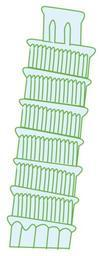
\includegraphics[scale=0.3]{pisa.jpg}};
      \draw[fill=gray] (0.2,-0.5) circle (0.1);
      \draw[fill=gray] (1,-0.5) circle (0.3);

    \end{tikzpicture}

    \vs

  \question
    A horse pulls a cart with a force of 400 Newtons forward.  However, according to Newton's Third Law, whenever the horse pulls the cart, there is an equal and opposite reaction of the cart pulling the horse.  Therefore, the cart pulls the horse with a force of 400 Newtons backward.  How does the cart move?  Shouldn't those two forces cancel each other out giving to a net force of zero?

    \tikzstyle{wheel}=[line width=10pt, fill=white]

    \begin{center}
      \begin{tikzpicture}[scale=0.5]
        \pingu[on horse,body=white, body front=white,small size, left eye color=white, right eye color=white,feet color=brown,bill color=white]
        \draw[rounded corners, fill=gray] 
          (0,-2) rectangle ++(7,-0.5);
        \draw[rounded corners, fill=gray] 
          (6,-1) -- ++(7,0) -- ++(-1,-4) -- ++(-5,0) -- cycle;
        \draw[wheel] (7,-5) circle (1);
        \draw[wheel] (12,-5) circle (1);
        \fill[pattern=north east lines] (-6,-6.3) rectangle ++(21, -0.5);
      \end{tikzpicture}
    \end{center}
    \vs[2]


  \pagebreak
  \question
    When do you are riding in an elevator, why do you sometimes feel heavier and why do you sometimes feel lighter?


    \def\headsize{0.4}
    \def\elevatorwidth{2.5}

    \tikzstyle{person}=[ultra thick, orange!50, scale=0.8]

    \tikzset{
      elevator/.pic = {
        \draw[fill=gray!30] 
          (-.2,-.05) rectangle (\elevatorwidth+.2,4.05);
        \draw[fill=white] 
          (0,0) rectangle (\elevatorwidth,4);

        %guide-line (for development)
        %\draw (\elevatorwidth/2,0) -- ++(0,4);


        \path (\elevatorwidth/2,4.4) coordinate (pulley);
        \draw (pulley) -- ++(0,-0.4);
        \filldraw[fill=gray] (pulley) circle (0.3);
        \filldraw[fill=gray!50] (pulley) circle (0.2);
        \draw[thick] (pulley) 
          ++(-0.3,1) --
          ++(0,-1)
          arc[start angle=-180, end angle=0, radius=0.3] --
          ++(0,1);
      }
    }


    \begin{center}
      \begin{tikzpicture}

        \begin{scope}
          \path (0,0) pic{elevator} coordinate (start);

          \begin{scope}[person]
            \draw (start) 
            ++(.95,0) coordinate (left foot) --
            ++(60:1.2) coordinate (waist) --
            ++(-60:1.2) coordinate (right foot);

            \draw (waist)
              -- ++(90:1.5) coordinate (neck);
            \draw (neck) 
              ++(90:\headsize) circle (\headsize);
            \draw (neck)
              -- ++(-70:0.7) coordinate (right elbow)
              -- ++(-100:0.5) coordinate (right hand);
            \draw (neck)
              -- ++(-110:0.7) coordinate (left elbow)
              -- ++(-80:0.5) coordinate (left hand);
          \end{scope}

          \draw (start) ++(\elevatorwidth/2,-0.5)
            node {\footnotesize stationary elevator};

        \end{scope}

        \begin{scope}
          \path (4.2,0) pic{elevator} coordinate (start);


          \begin{scope}[person]
            \draw (start) 
            ++(1.2,0) coordinate (left foot) --
            ++(110:0.6) --
            ++(20:0.6) coordinate (waist) --
            ++(-20:0.6) --
            ++(250:0.6) coordinate (right foot);


            \draw (waist)
              -- ++(90:1.5) coordinate (neck);
            \draw (neck) 
              ++(90:\headsize) circle (\headsize);
            \draw (neck)
              -- ++(-10:0.7) coordinate (right elbow)
              -- ++(10:0.5) coordinate (right hand);
            \draw (neck)
              -- ++(190:0.7) coordinate (left elbow)
              -- ++(170:0.5) coordinate (left hand);
          \end{scope}

          \draw (start) ++(\elevatorwidth/2,-0.5)
            node {\footnotesize accelerating upward};

        \end{scope}

        \begin{scope}
          \path (8.4,0) pic{elevator} coordinate (start);

          \begin{scope}[person]
            \draw (start) 
            ++(1.2,0) coordinate (left foot) --
            ++(75:1.2) coordinate (waist) --
            ++(-20:1.2) coordinate (right foot);

            \draw (waist)
              -- ++(100:1.5) coordinate (neck);
            \draw (neck) 
              ++(100:\headsize) circle (\headsize);
            \draw (neck)
              -- ++(10:0.7) coordinate (right elbow)
              -- ++(80:0.5) coordinate (right hand);
            \draw (neck)
              -- ++(-160:0.7) coordinate (left elbow)
              -- ++(110:0.5) coordinate (left hand);
          \end{scope}

          \draw (start) ++(\elevatorwidth/2,-0.5)
            node {\footnotesize accelerating downward};

        \end{scope}

      \end{tikzpicture}
    \end{center}

\end{questions}

\end{document}